\documentclass[handout]{beamer}

\usepackage{Haust2017glærur}

\title{Stærðfræðimynstur í tölvunarfræði}
\subtitle{Vika 9, seinni fyrirlestur}

\begin{document}

\begin{frame}
\titlepage
\end{frame}


\section{Inngangur}

\begin{frame}{Í síðasta tíma}
    \begin{itemize}
        \item Upprifjun á rakningarvenslum
        \item Endurkvæmni
        \item Endurkvæm reiknirit
    \end{itemize}
\end{frame}

\section{Kvik bestun}

\begin{frame}{Endurteknir útreikningar}
Ýmis endurkvæm reiknirit láta okkur reikna sömu stærðina oftar en einu sinni. Fibonacci-reikniritið úr kafla 5 er dæmi um slíkt:
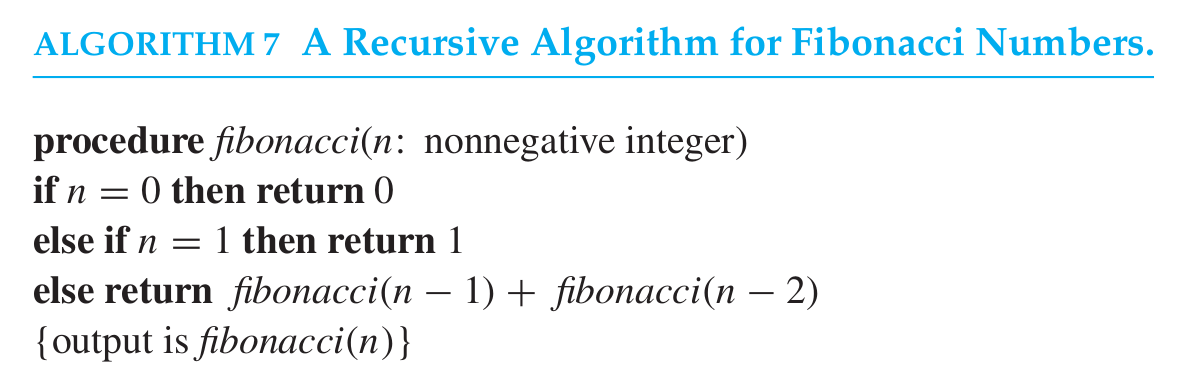
\includegraphics[width=\textwidth]{fibonacci-algorithm}

Endurteknir útreikningar haft mjög slæm áhrif á keyrslutíma forrits.
\end{frame}

\begin{frame}{Endurteknir útreikningar}
\begin{center}
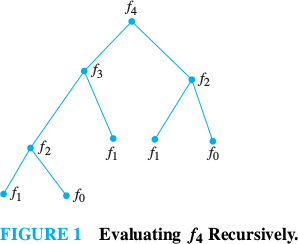
\includegraphics[width=0.6\textwidth]{fibonacci-execution}
\end{center}
\end{frame}

\begin{frame}{Kvik bestun}
    \begin{itemize}
        \item Til að forðast endurtekna útreikninga í endurkvæmu reikniriti má notast við kvika bestun (e. \emph{dynamic programming})
        \item Hugmyndin á bak við kvika bestun er brjóta vandamál endurkvæmt niður í smærri vandamál
        \begin{itemize}
            \item Reikna svo út niðurstöðu fyrir smáu tilvikin
            \item Komi smátt tilvik af vandamálinu fyrir aftur, þá má nýta geymdu niðurstöðuna
        \end{itemize}
        \item Kemur oft fyrir í bestunarvandamálum
        \begin{itemize}
            \item Nafnið ``dynamic programming'' kemur frá Richard Bellman
        \end{itemize}
    \end{itemize}
\end{frame}

\begin{frame}[fragile]{Skárra fibonacci-reiknirit}
\begin{columns}
\column{0.3\textwidth}
Notum ``utanáliggjandi geymslu'' til að halda utan um gildi sem þegar hafa verið reiknuð. Hér er geymslan vörpun frá $N$ til $N$.
\column{0.7\textwidth}
\begin{verbatim}
reiknirit fib(n: ekki-neikvæð heiltala)
  ef fib(n) er í geymslu:
    skila gildi úr geymslunni
  annars ef n==0:
    skila 1
  annars ef n==1:
    skila 1
  annars
    f := fib(n-1) + fib(n-2)
    setja f í geymslu
    skila f
\end{verbatim}
\end{columns}
\end{frame}

\section{Lausnir á rakningarvenslum}

\begin{frame}{Lausnir á rakningarvenslum}
\begin{itemize}
 \item Hingað til höfum við leyst rakningarvensl með því að skoða fyrstu liðina í runu sem uppfyllir venslin og sjá mynstur
 \item Við getum gert aðeins betur, en til þess þurfum við betri skilgreiningar
\end{itemize}
\end{frame}

\begin{frame}{Skilgreining}
\begin{tcolorbox}[title=Línuleg einsleit rakningarvensl með fastastuðlum]
Línuleg einsleit rakningarvensl (e. \emph{a linear homogeneous recurrence relation}) af stigi $k$ með fastastuðla eru rakningarvensl á eftirfarandi sniði:
\[
 a_n = c_1 a_{n-1} + c_2a_{n-2} + \ldots + c_ka_{n-k}
\]
þar sem $c_1, c_2, \ldots, c_k$ eru rauntölur, með $c_k \neq 0$.
\end{tcolorbox}
\begin{itemize}
 \item Rakningarvenslin eru línuleg af því hægri hlið jöfnunnar er einföld summa af fyrri liðum
 \item Rakningarvenslin eru einsleit því allir liðir hægri hliðarinnar eru fast margfeldi einhvers $a_j$
\end{itemize}
\end{frame}

\begin{frame}{Dæmi}
\begin{itemize}[<+->]
 \item Hvert er stig línulegu einsleitu rakningarvenslanna $P_n = 1.11P_{n-1}$?
 \begin{itemize}
  \item Stigið er 1, hver liður veltur á einum fyrri lið
 \end{itemize}
 \item Hvert er stig línulegu einsleitu rakningarvenslanna $f_n = f_{n-1} + f_{n-2}$?
 \begin{itemize}
  \item Stigið er 2
 \end{itemize}
 \item Hvert er stig línulegu einsleitu rakningarvenslanna\\ $a_n = a_{n-5}$?
 \begin{itemize}
  \item Stigið er 5
 \end{itemize}
\end{itemize}
\end{frame}

\begin{frame}{Dæmi}
\begin{itemize}
 \item Nokkur rakningarvensl sem eru ekki línuleg einsleit rakningarvensl með fastastuðla
 \begin{itemize}[<+->]
  \item $a_n = a_{n-1} + a_{n-2}^2$
  \begin{itemize}
   \item ekki línuleg
  \end{itemize}
  \item $H_n = 2H_{n-1} + 1$
  \begin{itemize}
   \item Ekki einsleit
  \end{itemize}
  \item $B_n = nB_{n-1}$
  \begin{itemize}
   \item Ekki með fastastuðla
  \end{itemize}
 \end{itemize}
\end{itemize}
\end{frame}

\begin{frame}{Að finna lausnir}
Þegar við leitum að runu sem á að uppfylla línuleg einsleit rakningarvensl með fastastuðla erum við venjulega að leita að runu með liði á sniðinu $a_n = r^n$, þar sem $r$ er fasti. Hægt er að sýna að runa með $a_n = r^n$ er lausn á venslunum $ a_n = c_1 a_{n-1} + \ldots + c_ka_{n-k}$ ef og aðeins ef
\[
 r^n = c_1r^{n-1} + c_2r^{n-2} + \ldots + c_kr^{n-k}
\]
. Deilum í gegn með $r^{n-k}$ og fáum jafngildu jöfnuna
\[
 r^k - c_1r^{k-1} - c_2r^{k-2} - \ldots - c_{k-1}r - c_k = 0
\]
. Við köllum síðustu jöfnuna kennijöfnu (e. \emph{characteristic equation}) rakningarvenslanna.
\end{frame}

\begin{frame}{Setning}
Skoðum sérstaklega lausnir á línulegum einsleitum rakningarvenslum af stigi 2:
\begin{tcolorbox}[title=Lausn einfaldra rakningarvensla af stigi 2]
Látum $c_1$ og $c_2$ vera rauntölur og að $r^2 - c_1r - c_2 = 0$ hafi tvær aðskildar rætur $r_1$ og $r_2$. Þá er runan $\{a_n\}$ lausn á rakningarvenslunum $a_n = c_1a_{n-1} + c_2a_{n-2}$ ef og aðeins ef $a_n = \alpha_1r_1^n + \alpha_2r^n_2$ fyrir $n=0,1,2,\ldots$ og $\alpha_1$ og $\alpha_2$ eru fastar.
\end{tcolorbox}

\end{frame}

\begin{frame}{Dæmi: Fibonacci}
    Finnum formúlu fyrir $n$-tu Fibonacci-töluna. \pause
    
    $n$-ta Fibonacci-talan er gefin með $f_n = f_{n-1} + f_{n-2}$, sem hefur kennijöfnuna $r^2 - r - 1 = 0$ með ræturnar 
    \[r_1 = \frac{1 + \sqrt{5}}{2} \]
    og
    \[r_2 = \frac{1 - \sqrt{5}}{2}\]
    svo
    \[
     f_n = \alpha_1\left(\frac{1 + \sqrt{5}}{2}\right)^n + \alpha_2\left(\frac{1 - \sqrt{5}}{2}\right)^n
    \]
\end{frame}
    
\begin{frame}{Dæmi: Fibonacci}
    Reiknum $\alpha_1$ og $\alpha_2$ út frá upphafsskilyrðunum $f_0 = 0$ og $f_1 = 1$:
    \begin{align*}
    f_0 &= \alpha_1 + \alpha_2 = 0\\
    f_1 &= \alpha_1\left(\frac{1 + \sqrt{5}}{2}\right) + \alpha_2\left(\frac{1 - \sqrt{5}}{2}\right) = 1
    \end{align*}
    og fáum $\alpha_1 = \frac{1}{\sqrt{5}}$, $\alpha_2 = -\frac{1}{\sqrt{5}}$, svo
    \[
     f_n = \frac{1}{\sqrt{5}}\left(\frac{1 + \sqrt{5}}{2}\right)^n -\frac{1}{\sqrt{5}}\left(\frac{1 - \sqrt{5}}{2}\right)^n
    \]
\end{frame}

\begin{frame}{Annað dæmi}
Getum við fundið lausn á rakningarvenslunum $a_n = a_{n-1} + 2a_{n-2}$ með upphafsskilyrðin $a_0 = 2$ og $a_1 = 7$? \pause

\vspace{0.5cm}
Já. Kennijafna rakningarvenslanna er $r^2 - r - 2 = 0$, með rætur $r_1 = 2$ og $r_2 = -1$. Þá er runan $\{a_n\}$ lausn á rakningarvenslunum ef og aðeins ef $a_n = \alpha_12^n + \alpha_2(-1)^n$ fyrir einhverja fasta $\alpha_1$ og $\alpha_2$.\pause

Upphafsskilyrðin gefa $a_0 = 2 = \alpha_1 + \alpha_2$ og $a_1 = 7 = \alpha_12 + \alpha_2(-1)$. Leysum þær og fáum $\alpha_1 = 3$ og $\alpha_2 = -1$. Þá er $\{a_n\}$ með

\[
 a_n = 3 \cdot 2^n - (-1)^n
\]
lausn á rakningarvenslunum.

\end{frame}

\begin{frame}{Fleiri setningar}
\begin{itemize}
 \item Setningin á fyrri glæru á einungis við línuleg einsleit rakningarvensl af stigi 2 með aðskildar rætur
 \begin{itemize}
  \item Það er ekki sérlega almennt
 \end{itemize}
 \item Í kafla 8.2 höfum við einnig\ldots
 \begin{itemize}
  \item setningu um línuleg einsleit rakningarvensl af stigi 2 með eina rót (Theorem 2)
  \item setningu um línuleg einsleit rakningarvensl af stigi $k$ með $k$ aðskildar rætur (Theorem 3)
  \item setningu um línuleg einsleit rakningarvensl af stigi $k$ með rætur sem geta verið endurteknar (Theorem 4)
  \item setningar um óeinsleit rakningarvensl (Theorem 5 og 6)
 \end{itemize}
\end{itemize}
\end{frame}

\section{Deila-og drottna reiknirit}

\begin{frame}{Deila-og-drottna reiknirit}
\begin{itemize}
 \item Mörg endurkvæm reiknirit fylgja svokallaðri deila-og-drottna (e. \emph{divide-and-conquer}) aðferðafræði
 \begin{itemize}
  \item Þau \emph{deila} vandamálinu niður í smærri tilvik af sjálfu sér
  \item Þau \emph{drottna} (yfir?) vandamálinu með því að nota smáu lausnirnar
 \end{itemize}
 \item Við getum notað rakningarvensl til að kanna tímaflækjur deila-og-drottna reiknirita
\end{itemize}
\end{frame}

\begin{frame}{Helmingunarleit}
    \begin{itemize}
        \item Helmingunarleit er klassískt deila-og-drottna reiknirit
        \item Skoðum fjölda samanburða sem við þurfum að framkvæma í helmingunarleit í $n$ staka runu
        \item Hvert skref í helmingunarleit minnkar stærð leitarbils úr $n$ niður í $\frac{n}{2}$ (ef $n$ er slétt)
        \item Í hverju skrefi framkvæmum við tvo samanburði
        \begin{itemize}
            \item Einn til að sjá hvorn helming rununnar við skoðum næst
            \item Einn til að sjá hvort við séum búin
        \end{itemize}
        \item Sé $b(n)$ fjöldi samanburða sem við þurfum til að leita að staki í runu af lengd $n$ fáum við þá
        \end{itemize}
        \[
        b(n) = b(n/2) + 2
        \]
\end{frame}

\begin{frame}{Skilvirk fylkjamargföldun}
    \begin{itemize}
        \item Strassen-reikniritið setur fylkjamargföldun á tveimur $n \times n$ fylkjum (þar sem $n$ er slétt) fram á nýjan hátt:
        \begin{itemize}
            \item Sjö margfaldanir á $\left(\frac{n}{2}\right)\times \left(\frac{n}{2}\right)$ fylkjum
            \item Fimmtán samlagningar á $\left(\frac{n}{2}\right)\times \left(\frac{n}{2}\right)$ fylkjum
        \end{itemize}
        \item Til þess þarf þá $f(n) = 7f(n/2) + 15n^2/4$ aðgerðir
    \end{itemize}
\end{frame}

\begin{frame}{Merge sort}
    \begin{itemize}
        \item Annað klassískt deila-og-drottna reiknirit er merge sort
        \item Hugmyndin að baki merge sort er eftirfarandi:
        \begin{itemize}
            \item Heildarrununni er skipt upp í tvær hlutrunur af jafnri (eða næstum jafnri) lengd
            \begin{itemize}
                \item Hverri hlutrunu er svo skipt upp í tvær hluthlutrunur, o.s.frv.
                \item Uppskiptingunni er haldið áfram þar til runurnar eru af lengdinni 1
            \end{itemize}
        \item Þegar uppskiptingunni er lokið eru runurnar sameinaðar tvær og tvær svo að úr verði röðuð runa
        \begin{itemize}
            \item Þegar síðustu sameiningunni er lokið er runan röðuð!
        \end{itemize}
        \item Merge sort var fundið upp af John von Neumann (1945)
        \end{itemize}
    \end{itemize}
\end{frame}

\begin{frame}{Keyrsla merge sort}
\vspace{0.5cm}
\begin{center}
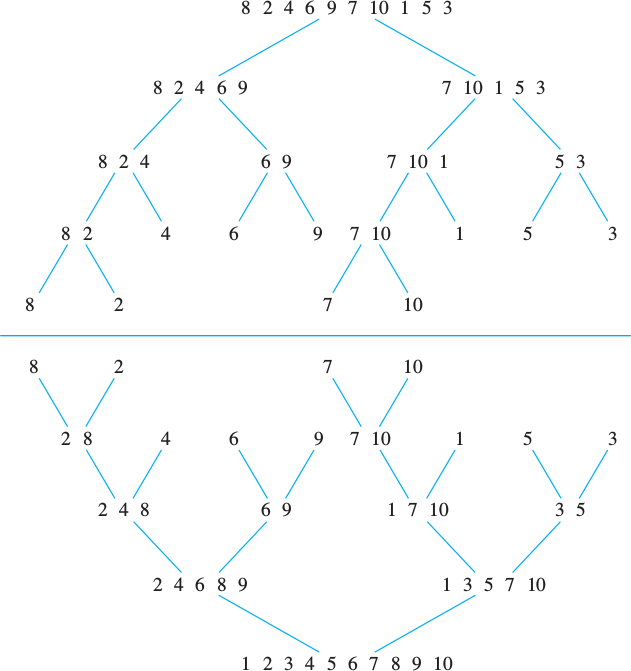
\includegraphics[width=0.5\textwidth]{merge-sort-visual}
\end{center}
\end{frame}

\begin{frame}{Merge reikniritið}
Mikið af vinnunni sem fer fram í merge sort felst í því að sameina listana:
\begin{center}
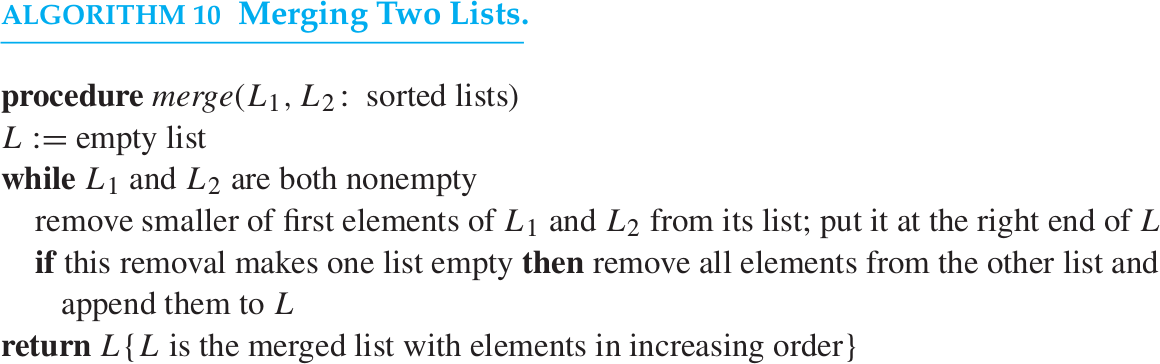
\includegraphics[width=\textwidth]{merge}
\end{center}
\end{frame}

\begin{frame}{Merge sort}
Merge sort er síðan lýst endurkvæmt:
\begin{center}
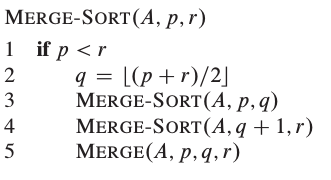
\includegraphics[width=0.9\textwidth]{merge-sort}
\end{center}
\end{frame}

\begin{frame}{Merge sort}
\begin{itemize}
 \item Merge sort skiptir runu af lengd $n$ sem raða skal endurtekið í hlutrunur af lengd $n/2$
 \begin{itemize}
  \item Síðan eru minna en $n$ samanburðir notaðir til að sameina hlutrunurnar tvær
 \end{itemize}
 \item Þá getum við lýst fjölda samanburða sem þarf til að raða $n$ staka runu með merge sort með fallinu $M(n)$,
\end{itemize}
\[
 M(n) = 2M(n/2) + n
\]
\end{frame}

\section{Tímaflækjur deila-og-drottna reiknirita}

\begin{frame}{Setning}
\begin{center}
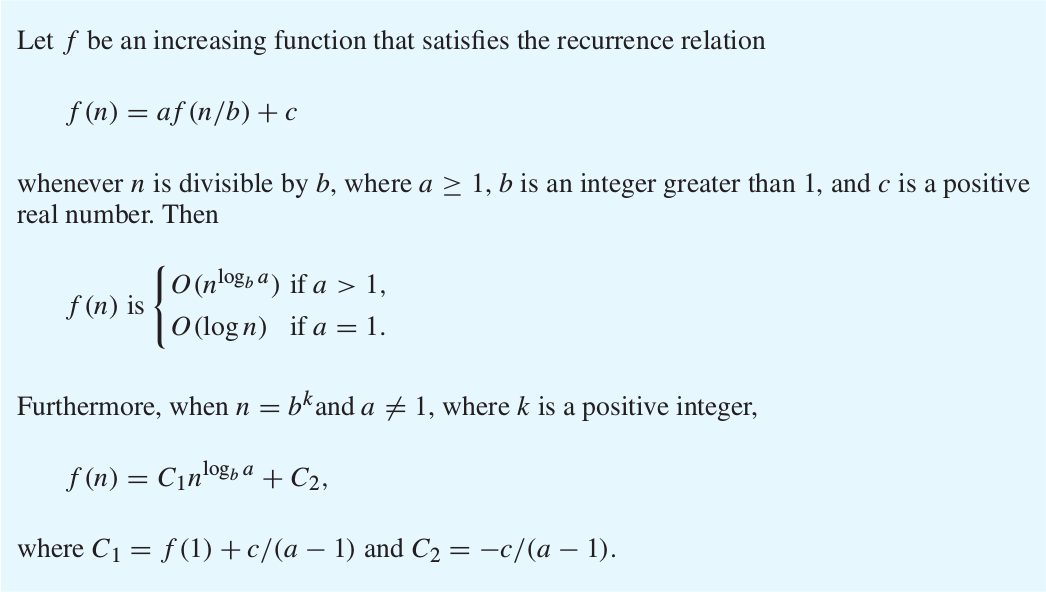
\includegraphics[width=\textwidth]{divide-and-conquer-time}
\end{center}
\end{frame}

\begin{frame}{Dæmi}
Fjöldi samanburða í helmingunarleit var $b(n) = b(n/2) + 2$ þegar $n$ er slétt tala. Hver er tímaflækja helmingunarleitar á stóra-O sniði? \pause

\vspace{1cm}
Skoðum setningu á fyrri glæru. Hér er $a=1$ svo helmingunarleit er $O(\log(n))$ reiknirit, sem passar við fyrri áætlanir.
\end{frame}

\begin{frame}{Öflugri setning}
Til að finna tímaflækjur reiknirita á borð við merge sort þurfum við öflugri setningu. Slík setning er:

\begin{center}
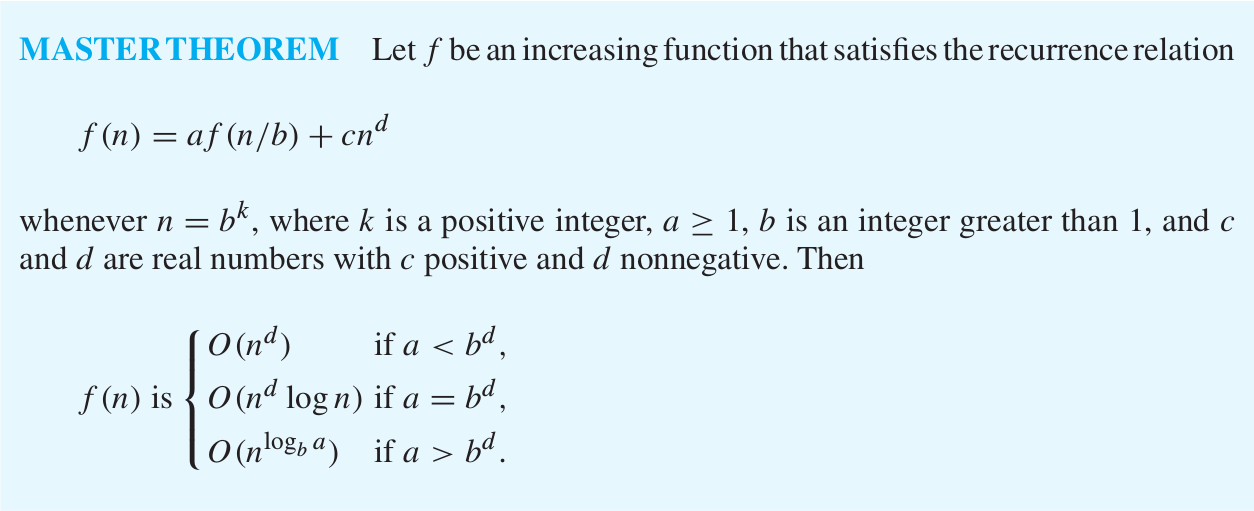
\includegraphics[width=\textwidth]{master-theorem}
\end{center}
\end{frame}

\begin{frame}{Dæmi}
Fjöldi samanburða í merge sort var $M(n) = 2M(n/2) + n$. Notum ``master theorem'' til að finna tímaflækju á stóra-O sniði.

\vspace{1cm}
Berum saman við $f(n) = af(n/b) + cn^d$ í master theorem. Sjáum að fallið sem lýsir fjölda samanburða passar sé $b=2$, $c=1$, $d=1$, $a=2=b^d$, svo við fáum að tímaflækjan sé $O(n^d\log (n)) = O(n\log(n))$ sem passar við fyrri áætlanir.
\end{frame}

\begin{frame}{Næst}
Net (byrjum á 10. kafla)
\end{frame}



\end{document}
